\documentclass[11pt,a4paper]{article}
\usepackage[utf8]{inputenc}
\usepackage[T1]{fontenc}
\usepackage[brazil]{babel}
\usepackage{amsmath,amssymb,amsfonts}
\usepackage{graphicx}
\usepackage[margin=2.2cm]{geometry}
\usepackage{booktabs}
\usepackage{enumitem}
\usepackage{tikz}
\usetikzlibrary{arrows.meta,positioning,calc}
\usepackage{hyperref}
\usepackage{xcolor}

\newcommand{\Lap}{\mathcal{L}}
\newcommand{\atan}{\operatorname{tg}^{-1}}
\tikzset{
  block/.style={draw, rectangle, minimum height=2.4em, minimum width=4.2em, fill=blue!4},
  sum/.style={draw, circle, minimum size=1.6em, inner sep=0pt},
  arr/.style={-{Latex[length=2mm]}},
}

\title{\textbf{Quarto Exerc\'icio Avaliativo de Sistemas de Controle}\\[2mm]
\large Resolu\c{c}\~ao detalhada}
\author{}
\date{07/07/2026}

\begin{document}
\maketitle

\noindent\textbf{Observa\c{c}\~oes gerais.} Nota\c{c}\~ao: $\sigma=\zeta\omega_n$,
$\omega_d=\omega_n\sqrt{1-\zeta^2}$. As refer\^encias usadas s\~ao
Franklin, Powell \& Emami-Naeini (FPE), \emph{Feedback Control of Dynamic Systems},
caps.~4--7, e Skogestad \& Postlethwaite, \emph{Multivariable Feedback Control} (Quest\~ao~4).
Os projetos das Quest\~oes 2 e 4 foram verificados numericamente (Python/SciPy);
as figuras de resposta ao degrau e lugar das ra\'izes foram geradas dessas verifica\c{c}\~oes.

%=====================================================================
\section*{Quest\~ao 1 --- Servomotor}

O servomotor \'e descrito por
\[
\ddot{\theta}+\dot{\theta}=u .
\]
Escolhendo os estados $x_1=\theta$ e $x_2=\dot{\theta}$, obt\'em-se a representa\c{c}\~ao
\[
\dot{x}=Ax+Bu,\qquad y=Cx,\qquad
A=\begin{bmatrix}0&1\\0&-1\end{bmatrix},\quad
B=\begin{bmatrix}0\\1\end{bmatrix},\quad
C=\begin{bmatrix}1&0\end{bmatrix}.
\]
A matriz de controlabilidade \'e
$\mathcal{C}=[\,B\;\;AB\,]=\begin{bmatrix}0&1\\1&-1\end{bmatrix}$, com
$\det\mathcal{C}=-1\neq0$: o sistema \'e control\'avel e podemos alocar os autovalores
livremente. A observabilidade tamb\'em vale:
$\mathcal{O}=\begin{bmatrix}C\\CA\end{bmatrix}=\begin{bmatrix}1&0\\0&1\end{bmatrix}$,
$\det\mathcal{O}=1\neq0$.

\subsection*{(a) Realimenta\c{c}\~ao de estados com autovalores em $-1$}

Com $u=Fx+r$, $F=[\,f_1\;\;f_2\,]$:
\[
A+BF=\begin{bmatrix}0&1\\ f_1 & -1+f_2\end{bmatrix},
\qquad
\det\!\big(sI-(A+BF)\big)=s^2+(1-f_2)s-f_1 .
\]
Queremos ambos os autovalores em $s=-1$, isto \'e, polin\^omio desejado
$(s+1)^2=s^2+2s+1$. Igualando coeficientes:
\[
1-f_2=2\;\Rightarrow\;f_2=-1,
\qquad
-f_1=1\;\Rightarrow\;f_1=-1 .
\]
\[
\boxed{\;F=[\,-1\;\;-1\,],\qquad u=-\theta-\dot{\theta}+r\;}
\]

\subsection*{(b) Otimalidade de $F$ (LQR)}

O funcional dado \'e
\[
J=\int_0^\infty\!\Big[\theta^2+\dot{\theta}^2+u^2\Big]dt
 =\int_0^\infty\!\big[x^{\!\top}Qx+u^{\!\top}Ru\big]dt,
\qquad Q=I_2,\;\;R=1 .
\]
O ganho \'otimo \'e $u=-R^{-1}B^{\!\top}P\,x$, onde $P=P^{\!\top}>0$ resolve a
equa\c{c}\~ao alg\'ebrica de Riccati (ARE)
\[
A^{\!\top}P+PA-PBR^{-1}B^{\!\top}P+Q=0 .
\]
Com $P=\begin{bmatrix}p_1&p_2\\p_2&p_3\end{bmatrix}$, calculamos termo a termo:
\[
A^{\!\top}P=\begin{bmatrix}0&0\\ p_1-p_2 & p_2-p_3\end{bmatrix},
\qquad
PA=(A^{\!\top}P)^{\!\top},
\qquad
PBB^{\!\top}P=\begin{bmatrix}p_2^2 & p_2p_3\\ p_2p_3 & p_3^2\end{bmatrix}.
\]
As tr\^es equa\c{c}\~oes escalares da ARE ficam:
\begin{align*}
(1,1):&\quad -p_2^2+1=0 &&\Rightarrow\; p_2=1 \;(\text{raiz}>0),\\
(2,2):&\quad 2(p_2-p_3)-p_3^2+1=0 \;\Rightarrow\; p_3^2+2p_3-3=0 &&\Rightarrow\; p_3=1 \;(\text{raiz}>0),\\
(1,2):&\quad (p_1-p_2)-p_2p_3=0 &&\Rightarrow\; p_1=p_2+p_2p_3=2 .
\end{align*}
\[
P=\begin{bmatrix}2&1\\1&1\end{bmatrix}>0
\quad(\text{menores principais }2>0,\ \det P=1>0),
\]
\[
F_{\mathrm{LQR}}=-R^{-1}B^{\!\top}P=-[\,p_2\;\;p_3\,]=[\,-1\;\;-1\,]=F .
\]
Ou seja, o ganho obtido em (a) \'e exatamente o ganho LQR com $Q=I$, $R=1$:
\emph{$F$ \'e \'otimo} e o custo m\'inimo vale $J^\ast=x(0)^{\!\top}Px(0)$.
(Coer\^encia: os polos \'otimos s\~ao as ra\'izes de $s^2+2s+1$, i.e.\ $\{-1,-1\}$,
os mesmos de (a).)

\subsection*{(c) Estimador (observador) assint\'otico de estados}

Como s\'o $\theta=y$ \'e medido, usamos o observador de Luenberger
\[
\dot{\hat{x}}=A\hat{x}+Bu+L\,(y-C\hat{x}),\qquad L=\begin{bmatrix}l_1\\l_2\end{bmatrix}.
\]
O erro de estima\c{c}\~ao $e=x-\hat{x}$ obedece $\dot e=(A-LC)e$, com
\[
A-LC=\begin{bmatrix}-l_1&1\\-l_2&-1\end{bmatrix},
\qquad
\det\!\big(sI-(A-LC)\big)=s^2+(1+l_1)s+(l_1+l_2).
\]
Escolhemos os polos do observador $4$--$5\times$ mais r\'apidos que os da malha de
controle ($-1,-1$), por exemplo ambos em $s=-5$:
$(s+5)^2=s^2+10s+25$. Igualando,
\[
1+l_1=10\Rightarrow l_1=9,\qquad l_1+l_2=25\Rightarrow l_2=16
\qquad\Longrightarrow\qquad
\boxed{L=\begin{bmatrix}9\\16\end{bmatrix}}
\]
e $e(t)\to0$ com constante de tempo $0{,}2$~s, bem antes da din\^amica dominante.

\subsection*{(d) Malha adicional para erro nulo a refer\^encias em degrau}

Com $u=Fx+r$ a fun\c{c}\~ao de transfer\^encia nominal \'e
$Y(s)/R(s)=1/(s+1)^2$, cujo ganho DC \'e 1 --- o erro nominal a degrau j\'a \'e zero.
Por\'em esse cancelamento \emph{n\~ao \'e robusto}: qualquer erro de modelo ou
perturba\c{c}\~ao constante gera erro de regime. A solu\c{c}\~ao cl\'assica \'e
\emph{a\c{c}\~ao integral} (FPE, se\c{c}.~7.10): acrescenta-se o estado
\[
\dot{x}_I=r-y=r-x_1,
\qquad
u=f_1x_1+f_2x_2+k_I\,x_I .
\]
A din\^amica aumentada em malha fechada \'e
\[
\frac{d}{dt}\!\begin{bmatrix}x_1\\x_2\\x_I\end{bmatrix}
=\begin{bmatrix}0&1&0\\ f_1& f_2-1 & k_I\\ -1&0&0\end{bmatrix}
\begin{bmatrix}x_1\\x_2\\x_I\end{bmatrix}
+\begin{bmatrix}0\\0\\1\end{bmatrix}r ,
\]
com polin\^omio caracter\'istico (expandindo o determinante pela terceira linha)
\[
\det(sI-A_{\mathrm{mf}})=s^3+(1-f_2)s^2-f_1s+k_I .
\]
Alocando os polos em $\{-1,-1,-2\}$, isto \'e,
$(s+1)^2(s+2)=s^3+4s^2+5s+2$:
\[
1-f_2=4\Rightarrow f_2=-3,\qquad
-f_1=5\Rightarrow f_1=-5,\qquad
k_I=2 .
\]
\[
\boxed{\;u=-5\theta-3\dot\theta+2\!\int_0^t\!\big(r-\theta\big)d\tau\;}
\]
O integrador garante $y(\infty)=r$ para degraus \emph{mesmo com} erros de modelo e
perturba\c{c}\~oes constantes na entrada, pois em regime $\dot x_I=0\Rightarrow y=r$.

\subsection*{(e) Controle com estado estimado: sistema global}

Usando $u=F\hat{x}+r$ (ganho de (a), observador de (c)), o diagrama de blocos \'e:

\begin{center}
\begin{tikzpicture}[node distance=1.1cm and 1.2cm]
\node[sum] (s1) {$+$};
\node[block, right=of s1] (plant) {$\dot{x}=Ax+Bu$};
\node[right=1.5cm of plant] (y) {$y=\theta$};
\node[block, below=0.9cm of plant] (obs) {\shortstack{Observador\\ $\dot{\hat x}=A\hat x+Bu+L(y-C\hat x)$}};
\node[block, left=of obs] (F) {$F$};
\node[left=1.0cm of s1] (r) {$r$};
\draw[arr] (r) -- (s1);
\draw[arr] (s1) -- node[above]{$u$} (plant);
\draw[arr] (plant) -- node[above, pos=.4]{$y$} (y);
\draw[arr] ($(plant.east)+(0.7,0)$) |- (obs.east);
\draw[arr] ($(s1.east)+(0.35,0)$) |- ([yshift=3mm]obs.east);
\draw[arr] (obs) -- node[above]{$\hat{x}$} (F);
\draw[arr] (F) -| (s1);
\end{tikzpicture}
\end{center}

\textbf{Espa\c{c}o de estados global.} Nas coordenadas $(x,\,e)$ com $e=x-\hat x$:
\[
\frac{d}{dt}\!\begin{bmatrix}x\\ e\end{bmatrix}
=\underbrace{\begin{bmatrix}A+BF & -BF\\ 0 & A-LC\end{bmatrix}}_{A_{\mathrm{g}}}
\begin{bmatrix}x\\ e\end{bmatrix}
+\begin{bmatrix}B\\ 0\end{bmatrix}r,
\qquad
y=[\,C\;\;0\,]\begin{bmatrix}x\\ e\end{bmatrix},
\]
numericamente
\[
A_{\mathrm{g}}=
\begin{bmatrix}
0&1&0&0\\
-1&-2&1&1\\
0&0&-9&1\\
0&0&-16&-1
\end{bmatrix},
\qquad
B_{\mathrm{g}}=\begin{bmatrix}0\\1\\0\\0\end{bmatrix},
\qquad
C_{\mathrm{g}}=[\,1\;0\;0\;0\,].
\]
Pela estrutura bloco-triangular vale o \textbf{princ\'ipio da separa\c{c}\~ao}: os
autovalores globais s\~ao os do controlador $\cup$ os do observador,
\[
\Lambda=\{-1,-1\}\cup\{-5,-5\}\subset\mathbb{C}^- \quad\Rightarrow\quad
\text{sistema global assintoticamente est\'avel.}
\]

\textbf{Fun\c{c}\~ao de transfer\^encia.} Como $\dot e$ n\~ao depende de $r$,
os modos do observador s\~ao \emph{n\~ao control\'aveis} a partir de $r$ e cancelam
na fun\c{c}\~ao de transfer\^encia:
\[
\frac{Y(s)}{R(s)}=C\big(sI-A-BF\big)^{-1}B=\frac{1}{(s+1)^2}.
\]
\'E \'util tamb\'em a fun\c{c}\~ao de transfer\^encia do \emph{compensador din\^amico}
equivalente (de $y$ para $u$, com $r=0$): de
$\dot{\hat x}=(A+BF-LC)\hat x+Ly$ e $u=F\hat x$,
\[
A+BF-LC=\begin{bmatrix}-9&1\\-17&-2\end{bmatrix},
\qquad
\frac{U(s)}{Y(s)}=F\big(sI-A-BF+LC\big)^{-1}L
=-\,\frac{25(s+1)}{s^2+11s+35},
\]
um compensador est\'avel (polos em $-5{,}5\pm j2{,}18$) cujo zero em $-1$ cancela o
polo est\'avel da planta $1/[s(s+1)]$ --- estrutura t\'ipica de projeto por observador.

\textbf{Controlabilidade/observabilidade.} O sistema global de 4\textsuperscript{a}
ordem \emph{n\~ao \'e completamente control\'avel} por $r$ (os modos $\{-5,-5\}$ do
erro s\~ao inating\'iveis --- por isso somem da FT), mas \'e
\emph{estabiliz\'avel} (os modos n\~ao control\'aveis s\~ao est\'aveis). Ele \'e
observ\'avel de $y$: o erro $e$ excita $x$ atrav\'es de $-BFe$ e $x_1$ \'e medido,
de modo que todos os quatro modos aparecem na sa\'ida. Em resumo: realiza\c{c}\~ao
m\'inima da FT \'e s\'o $1/(s+1)^2$; os modos extras s\~ao est\'aveis e inofensivos.

%=====================================================================
\section*{Quest\~ao 2 --- P\^endulo invertido sobre carro}

Dados:
\[
\frac{\Theta(s)}{V(s)}=-\frac{1}{s^2-1},
\qquad
\frac{Y(s)}{V(s)}=\frac{s^2-1+\beta}{s^2\,(s^2-1)},
\qquad
\beta=\frac{3m_p}{4(m_c+m_p)} .
\]
Com a rela\c{c}\~ao de massas pedida, $m_c=2m_p$:
\[
\beta=\frac{3m_p}{4(2m_p+m_p)}=\frac{3m_p}{12m_p}=\frac14 .
\]

\subsection*{(a) Compensador $D(s)$ da malha do p\^endulo}

Com a malha interna $V=U+D(s)\Theta$ e $G_\theta=-1/(s^2-1)$:
\[
\Theta=G_\theta V=G_\theta\big(U+D\Theta\big)
\quad\Longrightarrow\quad
\frac{\Theta(s)}{U(s)}=\frac{G_\theta}{1-G_\theta D}.
\]
Tomando $D(s)=K\dfrac{s+a}{s+b}$ com o zero cancelando o polo \emph{est\'avel} da
planta em $s=-1$, i.e.\ $a=1$:
\[
G_\theta D=-\frac{K(s+1)}{(s-1)(s+1)(s+b)}=-\frac{K}{(s-1)(s+b)},
\]
\[
1-G_\theta D=\frac{(s-1)(s+b)+K}{(s-1)(s+b)}
\quad\Longrightarrow\quad
\frac{\Theta(s)}{U(s)}
=-\,\frac{s+b}{(s+1)\big[(s-1)(s+b)+K\big]} .
\]
Os ``demais polos'' s\~ao as ra\'izes de
\[
(s-1)(s+b)+K=s^2+(b-1)s+(K-b)\;\overset{!}{=}\;(s+3-j3)(s+3+j3)=s^2+6s+18 ,
\]
logo
\[
b-1=6\Rightarrow b=7,
\qquad
K-b=18\Rightarrow K=25 .
\]
\[
\boxed{\;D(s)=\frac{25\,(s+1)}{s+7}\;},
\qquad
\frac{\Theta(s)}{U(s)}=-\,\frac{s+7}{(s+1)\,(s^2+6s+18)} .
\]
(O polo em $-1$ permanece como polo de malha fechada por ser um cancelamento
zero--polo \emph{est\'avel}; os polos alocados s\~ao $-3\pm j3$, como pedido.)

\subsection*{(b) Fun\c{c}\~ao de transfer\^encia $U\to Y$ e lugar das ra\'izes}

Como $Y=G_y V$ e $V=U/(1-G_\theta D)$:
\[
\frac{Y(s)}{U(s)}=\frac{G_y(s)}{1-G_\theta(s) D(s)}
=\frac{s^2-\tfrac34}{s^2(s^2-1)}\cdot\frac{(s-1)(s+7)}{s^2+6s+18},
\]
e, cancelando $(s-1)$,
\[
\boxed{\;
P(s)\equiv\frac{Y(s)}{U(s)}
=\frac{(s+7)\left(s^2-\tfrac34\right)}{s^2\,(s+1)\,(s^2+6s+18)}
=\frac{(s+7)(s+0{,}866)(s-0{,}866)}{s^2(s+1)(s^2+6s+18)} \;}
\]
Portanto: $n=5$ polos $\{0,0,-1,-3\pm j3\}$ e $m=3$ zeros
$\{-7,\,\pm\sqrt{3}/2\approx\pm0{,}866\}$ --- note o \textbf{zero de fase
n\~ao m\'inima} em $s=+0{,}866$ e o ganho DC \emph{negativo}
($\lim_{s\to0}s^2P=-5{,}25/18<0$).

\emph{Esbo\c{c}o (regras de LGR):} $n-m=2$ ramos v\~ao para o infinito.
Para $K>0$ (LGR de $180^\circ$) as ass\'intotas s\~ao $\pm90^\circ$ com centroide
\[
\sigma_a=\frac{\sum p_i-\sum z_i}{n-m}
=\frac{(0+0-1-3-3)-(-7+0{,}866-0{,}866)}{2}=\frac{-7+7}{2}=0 ,
\]
i.e.\ sobre o eixo imagin\'ario; al\'em disso um ramo real \'e atra\'ido pelo zero em
$+0{,}866$: \emph{h\'a sempre polo no semiplano direito}. Para $K<0$
(LGR de $0^\circ$) os ramos do polo duplo na origem abrem ao longo do eixo real e um
deles caminha para o zero em $+0{,}866$: tamb\'em h\'a sempre um polo com
$\mathrm{Re}(s)>0$ (verificado numericamente: $\max\mathrm{Re}=+0{,}018$ em
$K=-0{,}1$, crescendo com $|K|$). A Figura~\ref{fig:q2rl} mostra os dois casos.

\textbf{Conclus\~ao do esbo\c{c}o:} \emph{nenhum ganho est\'atico estabiliza a malha
do carro} --- \'e necess\'aria compensa\c{c}\~ao din\^amica (itens (c)/(d)).

\begin{figure}[htb]
\centering
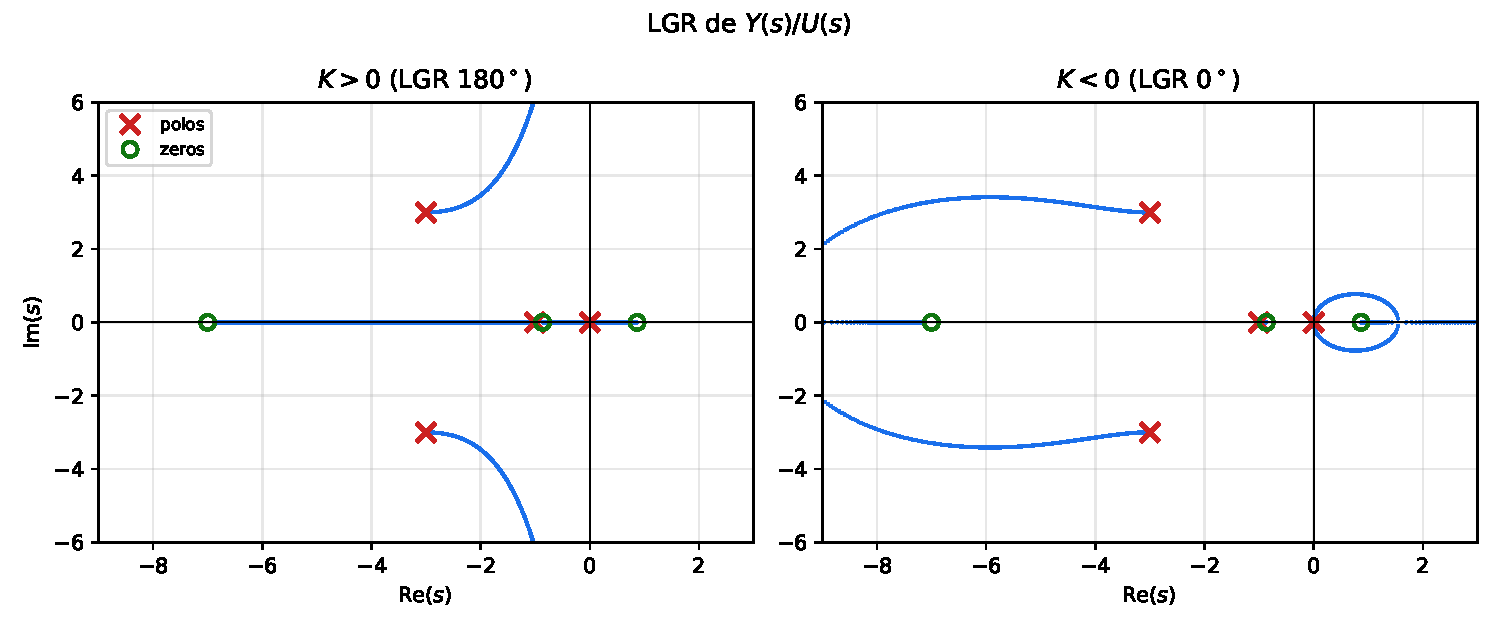
\includegraphics[width=.95\linewidth]{figs/q2_rlocus.pdf}
\caption{Lugar das ra\'izes de $P(s)=Y/U$ para ganho positivo e negativo.}
\label{fig:q2rl}
\end{figure}

\subsection*{(c) Diagrama de blocos com as duas malhas}

Como $Y/\Theta=\dfrac{Y/V}{\Theta/V}=-\dfrac{s^2-1+\beta}{s^2}$, o sistema pode ser
desenhado em cascata:

\begin{center}
\begin{tikzpicture}[node distance=0.9cm and 0.75cm]
\node (r) {$R$};
\node[sum, right=of r] (s1) {};
\node[block, right=of s1] (C) {$C(s)$};
\node[sum, right=of C] (s2) {};
\node[block, right=of s2] (Gt) {$-\dfrac{1}{s^2-1}$};
\node[block, right=1.1cm of Gt] (Gy) {$-\dfrac{s^2-\frac34}{s^2}$};
\node[right=0.9cm of Gy] (y) {$Y$};
\node[block, below=0.8cm of Gt] (D) {$D(s)=\dfrac{25(s+1)}{s+7}$};
\draw[arr] (r) -- (s1);
\draw[arr] (s1) -- node[above]{$e$} (C);
\draw[arr] (C) -- node[above]{$U$} (s2);
\draw[arr] (s2) -- node[above]{$V$} (Gt);
\draw[arr] (Gt) -- node[above]{$\Theta$} (Gy);
\draw[arr] (Gy) -- (y);
\draw[arr] ($(Gt.east)+(0.5,0)$) |- (D.east);
\draw[arr] (D.west) -| node[right, pos=.85]{$+$} (s2);
\draw[arr] ($(Gy.east)+(0.45,0)$) -- ++(0,-2.5) -| node[right, pos=.97]{$-$} (s1);
\node at ($(s1)+(0.32,0.3)$) {\small$+$};
\node at ($(s2)+(-0.3,0.3)$) {\small$+$};
\end{tikzpicture}
\end{center}

A malha interna ($D$) estabiliza o p\^endulo; a malha externa ($C$) controla a
posi\c{c}\~ao do carro realimentando $Y$.

\subsection*{(d) Projeto de $C(s)$ para $M_p<50\%$}

Requisitos estruturais vindos de (b): (i) o ganho de $C$ deve ser
\emph{negativo} (ganho DC de $P$ \'e negativo); (ii) \'e preciso um \emph{zero de
avan\c{c}o} perto da origem para puxar os dois ramos do polo duplo em $s=0$ para o
semiplano esquerdo (a\c{c}\~ao tipo PD); (iii) a banda passante deve ficar bem abaixo
do zero de fase n\~ao m\'inima em $0{,}866$~rad/s. Proponho o compensador de avan\c{c}o
\[
\boxed{\;C(s)=-2\,\frac{s+0{,}1}{s+2}\;}
\]
(zero uma d\'ecada abaixo do zero NMP; polo em $-2$ para realizabilidade). O ganho
$|K_c|=2$ foi ajustado no lugar das ra\'izes/simula\c{c}\~ao. O polin\^omio de malha
fechada $1+C(s)P(s)=0$ resulta nos polos
\[
\{-3{,}53\pm j2{,}88,\;\; -0{,}70\pm j0{,}51,\;\; -0{,}332,\;\; -0{,}203\}\subset\mathbb{C}^-,
\]
todos est\'aveis. A resposta ao degrau simulada (Fig.~\ref{fig:q2step}) d\'a
\[
M_p\approx32\%<50\%\;\checkmark,\qquad t_p\approx7{,}8\ \mathrm{s},\qquad
t_{s,5\%}\approx21\ \mathrm{s},
\]
com o \emph{sub-sinal inverso} inicial de ${\approx}21\%$ que \'e inevit\'avel: \'e a
assinatura do zero em $s=+0{,}866$ (o carro precisa recuar para inclinar o p\^endulo
na dire\c{c}\~ao do movimento).

\begin{figure}[htb]
\centering
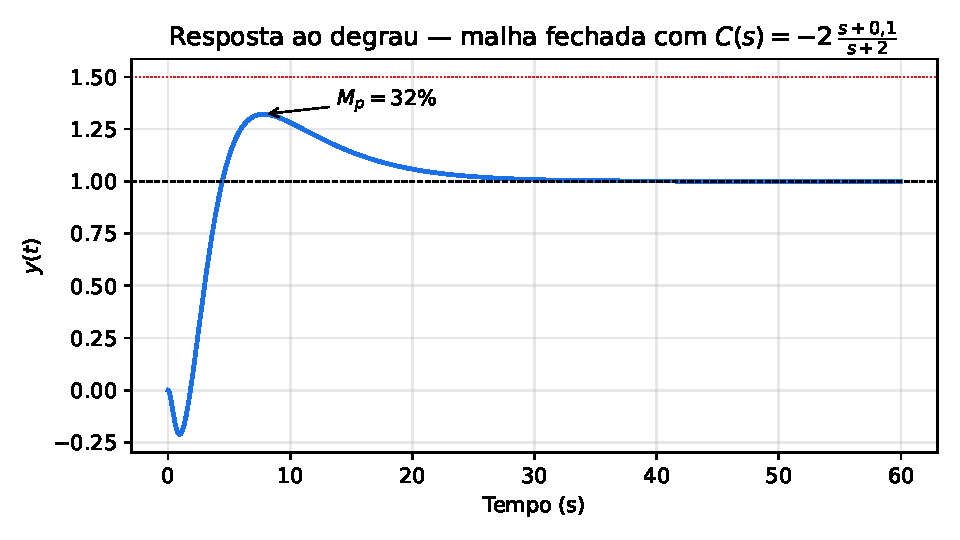
\includegraphics[width=.7\linewidth]{figs/q2_step.pdf}
\caption{Resposta ao degrau da malha fechada do carro com $C(s)=-2(s+0{,}1)/(s+2)$.}
\label{fig:q2step}
\end{figure}

\subsection*{(e) Erro em regime permanente}

O ganho de la\c{c}o $L(s)=C(s)P(s)$ cont\'em o fator $1/s^2$ (duplo integrador do
carro): o sistema \'e do \textbf{tipo 2}. Como a malha fechada \'e est\'avel,
pelo teorema do valor final, para $E=R/(1+L)$:
\[
e_{ss}^{\text{degrau}}=\lim_{s\to0}\frac{s\cdot\frac1s}{1+L(s)}=0,
\qquad
e_{ss}^{\text{rampa}}=0,
\qquad
e_{ss}^{\text{par\'abola}}=\frac{1}{K_a},
\]
com
\[
K_a=\lim_{s\to0}s^2L(s)
=C(0)\cdot\lim_{s\to0}s^2P(s)
=\Big(\!-2\cdot\tfrac{0{,}1}{2}\Big)\cdot\frac{7\cdot(-\tfrac34)}{18}
=\frac{7}{240}\approx0{,}029 .
\]
\[
\boxed{\;e_{ss}=0 \text{ para degrau (e rampa); } e_{ss}=240/7\approx34 \text{ para par\'abola.}\;}
\]

%=====================================================================
\section*{Quest\~ao 3 --- Segunda ordem com zero extra}

\[
H(s)=\frac{\omega_n^2\,(s+z)}{z\,\big(s^2+2\zeta\omega_n s+\omega_n^2\big)},
\qquad H(0)=1 .
\]

\subsection*{(a) Resposta ao degrau unit\'ario}

\textbf{Passo 1 --- decomposi\c{c}\~ao.} Escrevendo
\[
H(s)=\underbrace{\frac{\omega_n^2}{s^2+2\zeta\omega_n s+\omega_n^2}}_{H_0(s)}
\Big(1+\frac{s}{z}\Big)
\quad\Longrightarrow\quad
Y(s)=\frac{H(s)}{s}=\frac{H_0(s)}{s}+\frac1z\,H_0(s),
\]
ou seja, no tempo,
\[
y(t)=y_0(t)+\frac1z\,\dot y_0(t),
\]
onde $y_0$ \'e a resposta ao degrau do sistema de 2\textsuperscript{a} ordem
\emph{sem} zero. Da teoria cl\'assica (FPE, cap.~3), com $\sigma=\zeta\omega_n$ e
$\omega_d=\omega_n\sqrt{1-\zeta^2}$:
\[
y_0(t)=1-e^{-\sigma t}\Big(\cos\omega_d t+\frac{\sigma}{\omega_d}\sin\omega_d t\Big),
\qquad
\dot y_0(t)=\frac{\omega_n^2}{\omega_d}\,e^{-\sigma t}\sin\omega_d t .
\]

\textbf{Passo 2 --- soma.}
\[
y(t)=1-e^{-\sigma t}\Big[\cos\omega_d t
+\underbrace{\frac{\sigma-\omega_n^2/z}{\omega_d}}_{\textstyle B}\,\sin\omega_d t\Big].
\]
Definindo $\eta\equiv\omega_n/z$, o coeficiente $B$ simplifica para
\[
B=\frac{\zeta\omega_n-\omega_n^2/z}{\omega_n\sqrt{1-\zeta^2}}
=\frac{\zeta-\eta}{\sqrt{1-\zeta^2}}
=-\,\frac{\eta-\zeta}{\sqrt{1-\zeta^2}} .
\]

\textbf{Passo 3 --- forma amplitude--fase.} Usando
$\cos\psi+B\sin\psi=\sqrt{1+B^2}\,\cos(\psi+\beta_1)$ com $\tan\beta_1=-B$:
\[
\sqrt{1+B^2}
=\sqrt{1+\frac{(\eta-\zeta)^2}{1-\zeta^2}}
=\sqrt{\frac{1-\zeta^2+\eta^2-2\zeta\eta+\zeta^2}{1-\zeta^2}}
=\frac{\sqrt{1+\dfrac{\omega_n^2}{z^2}-\dfrac{2\zeta\omega_n}{z}}}{\sqrt{1-\zeta^2}} ,
\]
\[
\boxed{\;
y(t)=1-\frac{\sqrt{1+\frac{\omega_n^2}{z^2}-\frac{2\zeta\omega_n}{z}}}{\sqrt{1-\zeta^2}}\;
e^{-\sigma t}\cos\big(\omega_d t+\beta_1\big),
\qquad
\beta_1=\atan\!\frac{-\zeta+\frac{\omega_n}{z}}{\sqrt{1-\zeta^2}} \;}
\]
exatamente a express\~ao do enunciado. (Verifica\c{c}\~ao: com $z\to\infty$,
$\beta_1\to-\mathrm{sen}^{-1}\zeta$ e recupera-se a resposta cl\'assica sem zero;
a f\'ormula tamb\'em foi conferida contra simula\c{c}\~ao num\'erica, coincidindo em
4 casas decimais.)

\subsection*{(b) Sobressinal $M_p$}

Chamando $R=\sqrt{1+\eta^2-2\zeta\eta}\big/\sqrt{1-\zeta^2}$, derivamos:
\[
\dot y(t)=R\,e^{-\sigma t}\Big[\sigma\cos(\omega_d t+\beta_1)+\omega_d\sin(\omega_d t+\beta_1)\Big]=0
\quad\Longrightarrow\quad
\tan(\omega_d t+\beta_1)=-\frac{\sigma}{\omega_d}=-\frac{\zeta}{\sqrt{1-\zeta^2}} .
\]
O primeiro m\'aximo ocorre em
\[
\omega_d t_p+\beta_1=\pi-\varphi_0,
\qquad
\varphi_0\equiv\atan\frac{\zeta}{\sqrt{1-\zeta^2}}=\mathrm{sen}^{-1}\zeta ,
\]
\[
t_p=\frac{\pi-\varphi_0-\beta_1}{\omega_d} .
\]
Nesse instante $\cos(\omega_d t_p+\beta_1)=\cos(\pi-\varphi_0)=-\sqrt{1-\zeta^2}$, logo
\[
y(t_p)=1+R\sqrt{1-\zeta^2}\,e^{-\sigma t_p}
\quad\Longrightarrow\quad
\boxed{\;
M_p=\sqrt{1+\frac{\omega_n^2}{z^2}-\frac{2\zeta\omega_n}{z}}\;
\exp\!\Big[-\frac{\zeta}{\sqrt{1-\zeta^2}}\big(\pi-\mathrm{sen}^{-1}\zeta-\beta_1\big)\Big]\;}
\]
\emph{Verifica\c{c}\~ao de sanidade:} $z\to\infty\Rightarrow\beta_1\to-\mathrm{sen}^{-1}\zeta$
e $M_p\to e^{-\pi\zeta/\sqrt{1-\zeta^2}}$, a f\'ormula cl\'assica. Para $z$ finito
(zero no semiplano esquerdo, perto dos polos) o radical \'e $>1$ e $\beta_1>-\varphi_0$:
o zero \emph{aumenta} o sobressinal e \emph{antecipa} o pico.

\subsection*{(c) Rela\c{c}\~ao entre $M_p$, $\zeta$ e $\omega_n$}

A express\~ao acima mostra que $M_p$ depende \emph{apenas} do par
$\big(\zeta,\ \eta=\omega_n/z\big)$ --- e n\~ao de $\omega_n$ isoladamente.
Consequ\^encias pr\'aticas:
\begin{itemize}[itemsep=1pt]
\item Sem o zero, $M_p$ fixa $\zeta$ pela f\'ormula cl\'assica
$\zeta=\dfrac{-\ln M_p}{\sqrt{\pi^2+\ln^2 M_p}}$ e $\omega_n$ fica livre para atender
requisitos de velocidade ($t_r$, $t_s$).
\item Com o zero, para um dado $M_p$ h\'a uma \emph{curva} de pares
$(\zeta,\eta)$ solu\c{c}\~ao de $M_p(\zeta,\eta)=M_p^\ast$ (resolvida numericamente ou
por \'abacos). Como o zero aumenta $M_p$, \'e preciso \textbf{mais amortecimento}
que no caso cl\'assico.
\item Se o zero $z$ \'e fixo (imposto pela f\'isica), aumentar $\omega_n$ aumenta
$\eta=\omega_n/z$ e portanto o sobressinal: surge um \emph{compromisso}
velocidade~$\times$~sobressinal, e $\omega_n$ passa a ser limitado por cima.
\end{itemize}
Exemplo num\'erico (resolvendo $M_p=20\%$):
\begin{center}
\begin{tabular}{lcccc}
\toprule
$\eta=\omega_n/z$ & $0$ (sem zero) & $0{,}5$ & $1$ & $2$\\
\midrule
$\zeta$ necess\'ario & $0{,}456$ & $0{,}490$ & $0{,}594$ & $0{,}917$\\
\bottomrule
\end{tabular}
\end{center}
A Figura~\ref{fig:q3mp} ilustra $M_p(\zeta)$ para v\'arias posi\c{c}\~oes do zero.

\begin{figure}[htb]
\centering
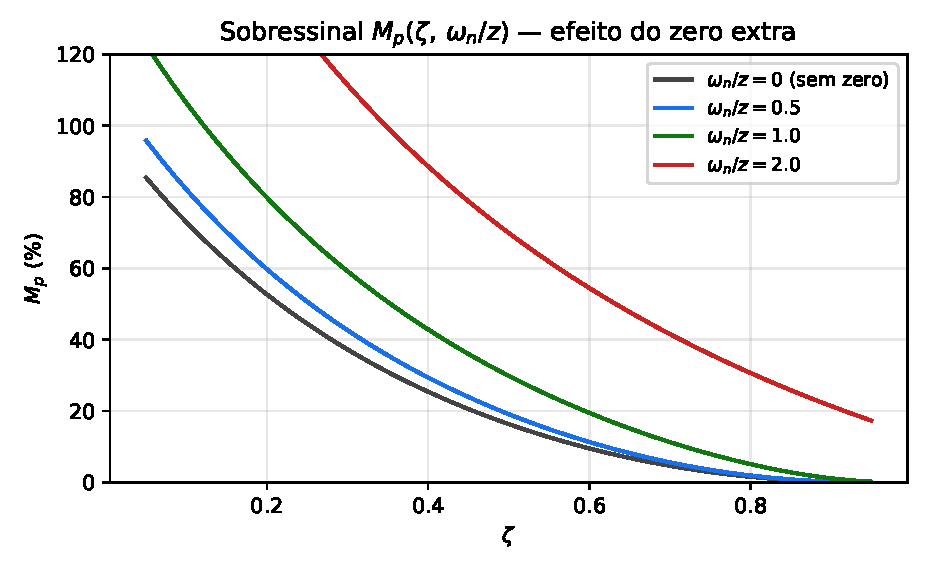
\includegraphics[width=.68\linewidth]{figs/q3_mp.pdf}
\caption{Efeito do zero extra sobre o sobressinal.}
\label{fig:q3mp}
\end{figure}

%=====================================================================
\section*{Quest\~ao 4 --- Processo industrial (v\'alvula, bomba e dois tanques)}

\textbf{Modelagem f\'isica (base para todos os itens).} Com \'area $A=1\ \mathrm{m^2}$
e a equa\c{c}\~ao de balan\c{c}o $A\dot h=\sum Q_{\mathrm{in}}-\sum Q_{\mathrm{out}}$,
e usando as hip\'oteses do enunciado (v\'alvula alimenta o tanque~1 com vaz\~ao $v_1$;
bomba transfere $v_2$ do tanque~1 para o tanque~2; a sa\'ida do tanque~2 \'e mantida
igual a $v_1$):
\[
\dot y_1=v_1-v_2,
\qquad
\dot y_2=v_2-v_1 .
\]
Note desde j\'a a \textbf{lei de conserva\c{c}\~ao}
$\dot y_1+\dot y_2=0$: \emph{o volume total \'e invariante}, pois tudo que entra no
tanque~1 sai do tanque~2 na mesma taxa. Essa propriedade estrutural domina os itens
(d), (e) e (g).

\subsection*{(a) Diagrama de blocos}

\begin{center}
\begin{tikzpicture}[node distance=0.8cm and 0.7cm]
% malha 1
\node (r1) {$r_1$};
\node[sum, right=of r1] (e1) {};
\node[block, right=of e1] (C1) {$C_1(s)$};
\node[block, right=of C1, fill=orange!10] (V) {\shortstack{V\'alvula\\ $G_v(s)$}};
\node[sum, right=1.0cm of V] (n1) {};
\node[block, right=of n1, fill=green!8] (T1) {\shortstack{Tanque 1\\ $\dfrac{1}{A s}$}};
\node[right=0.7cm of T1] (y1) {$y_1$};
% malha 2
\node[sum, below=2.1cm of e1] (e2) {};
\node[left=0.7cm of e2] (r2) {$r_2$};
\node[block, right=of e2] (C2) {$C_2(s)$};
\node[block, right=of C2, fill=orange!10] (Bm) {\shortstack{Bomba\\ $G_b(s)$}};
\node[sum, right=1.0cm of Bm] (n2) {};
\node[block, right=of n2, fill=green!8] (T2) {\shortstack{Tanque 2\\ $\dfrac{1}{A s}$}};
\node[right=0.7cm of T2] (y2) {$y_2$};
\draw[arr] (r1) -- (e1); \draw[arr] (e1) -- (C1);
\draw[arr] (C1) -- node[above]{$u_1$} (V);
\draw[arr] (V) -- node[above]{$v_1$} node[below, pos=.8]{\small$+$} (n1);
\draw[arr] (n1) -- (T1); \draw[arr] (T1) -- (y1);
\draw[arr] (r2) -- (e2); \draw[arr] (e2) -- (C2);
\draw[arr] (C2) -- node[above]{$u_2$} (Bm);
\draw[arr] (Bm) -- node[above]{$v_2$} node[below, pos=.8]{\small$+$} (n2);
\draw[arr] (n2) -- (T2); \draw[arr] (T2) -- (y2);
% cross couplings
\draw[arr] ($(Bm.east)+(0.4,0)$) -- ++(0,1.2) -| node[left, pos=.94]{\small$-$} (n1);
\draw[arr] ($(V.east)+(0.4,0)$) -- ++(0,-1.2) -| node[left, pos=.94]{\small$-$} (n2);
% feedbacks
\draw[arr] ($(T1.east)+(0.4,0)$) -- ++(0,1.15) -| node[right, pos=.97]{\small$-$} (e1);
\draw[arr] ($(T2.east)+(0.4,0)$) -- ++(0,-1.15) -| node[right, pos=.97]{\small$-$} (e2);
\node at ($(e1)+(-0.32,0.28)$) {\small$+$};
\node at ($(e2)+(-0.32,0.28)$) {\small$+$};
\end{tikzpicture}
\end{center}

Blocos distintos: controladores $C_1$, $C_2$; atuadores (v\'alvula $G_v$ e bomba
$G_b$); tanques (integradores $1/As$). As duas malhas descentralizadas e os
\emph{acoplamentos cruzados} ($v_2$ retira do tanque~1; $v_1$ \'e retirado do
tanque~2) ficam evidentes.

\subsection*{(b) Identifica\c{c}\~ao de $G_v(s)$ e $G_b(s)$ pelas respostas ao degrau}

Para um modelo de 1\textsuperscript{a} ordem $G(s)=K/(\tau s+1)$ e degrau
unit\'ario: $K$ \'e o valor final e $\tau$ \'e o instante em que a resposta atinge
$63{,}2\%$ do valor final. Lendo as Figuras 2 e 3 do enunciado:
\begin{itemize}[itemsep=1pt]
\item \textbf{V\'alvula (Fig.~2):} valor final $v_1(\infty)\approx2$; $63\%$ de 2
($\approx1{,}26$) ocorre em $t\approx10$~s; a resposta acomoda ($\approx98\%$)
perto de $4\tau\approx40$~s, coerente com o gr\'afico.
\item \textbf{Bomba (Fig.~3):} valor final $v_2(\infty)\approx2{,}5$; $63\%$
($\approx1{,}58$) em $t\approx2$~s; acomoda\c{c}\~ao em ${\approx}8$~s.
\end{itemize}
\[
\boxed{\;
G_v(s)=\frac{V_1(s)}{U_1(s)}=\frac{2}{10s+1},
\qquad
G_b(s)=\frac{V_2(s)}{U_2(s)}=\frac{2{,}5}{2s+1}\;}
\]
(valores lidos dos gr\'aficos; a metodologia \'e o que importa).

\subsection*{(c) Modelos entrada--sa\'ida e em espa\c{c}o de estados (malha aberta)}

\textbf{Entrada--sa\'ida.} De $\dot y_1=v_1-v_2$ e $\dot y_2=v_2-v_1$:
\[
\begin{bmatrix}Y_1(s)\\[1mm] Y_2(s)\end{bmatrix}
=\underbrace{\frac1s
\begin{bmatrix} G_v(s) & -G_b(s)\\[1mm] -G_v(s) & G_b(s)\end{bmatrix}}_{G(s)}
\begin{bmatrix}U_1(s)\\[1mm] U_2(s)\end{bmatrix}
=\frac1s\begin{bmatrix}\dfrac{2}{10s+1} & -\dfrac{2{,}5}{2s+1}\\[3mm]
-\dfrac{2}{10s+1} & \dfrac{2{,}5}{2s+1}\end{bmatrix}U(s) .
\]
Observe que
$G(s)=\frac1s\begin{bmatrix}1\\-1\end{bmatrix}\!\begin{bmatrix}G_v&-G_b\end{bmatrix}$
tem \textbf{posto~1 em toda frequ\^encia}: s\'o a combina\c{c}\~ao
$y_1-y_2$ \'e funcionalmente control\'avel; $y_1+y_2$ n\~ao responde \`as entradas.

\textbf{Espa\c{c}o de estados.} Estados $x=[\,v_1\;v_2\;y_1\;y_2\,]^{\!\top}$:
\[
\dot x=
\begin{bmatrix}
-\frac1{10}&0&0&0\\[1mm]
0&-\frac12&0&0\\[1mm]
1&-1&0&0\\[1mm]
-1&1&0&0
\end{bmatrix}x
+
\begin{bmatrix}
\frac{2}{10}&0\\[1mm]
0&\frac{2{,}5}{2}\\[1mm]
0&0\\[1mm]
0&0
\end{bmatrix}
\begin{bmatrix}u_1\\u_2\end{bmatrix},
\qquad
y=\begin{bmatrix}0&0&1&0\\0&0&0&1\end{bmatrix}x .
\]
Autovalores em malha aberta: $\{-0{,}1,\,-0{,}5,\,0,\,0\}$. Um dos modos nulos
($y_1+y_2$) \'e \emph{n\~ao control\'avel} --- \'e a lei de conserva\c{c}\~ao.

\subsection*{(d) Controladores proporcionais: para que ganhos h\'a estabilidade?}

Com $u_1=k_1(r_1-y_1)$ e $u_2=k_2(r_2-y_2)$, o polin\^omio caracter\'istico do
sistema em malha fechada fatora como (usando as coordenadas
$w=y_1+y_2$, $z=y_1-y_2$; $\dot w=0$ sempre):
\[
\Delta(s)=s\cdot p_3(s),
\qquad
p_3(s)=s^3+(a+b)s^2+\big(ab+2c_1+2c_2\big)s+2\big(a\,c_2+b\,c_1\big),
\]
onde
\[
a=\frac1{\tau_v}=0{,}1,\quad
b=\frac1{\tau_b}=0{,}5,\quad
c_1=\frac{K_vk_1}{2\tau_v}=0{,}1k_1,\quad
c_2=\frac{K_bk_2}{2\tau_b}=0{,}625\,k_2 .
\]
\textbf{Routh--Hurwitz em $p_3$:} para $s^3+a_2s^2+a_1s+a_0$ exige-se
$a_2>0$, $a_1>0$, $a_0>0$ e $a_2a_1>a_0$. Aqui $a_2=a+b>0$ sempre, e
\[
a_2a_1-a_0=(a+b)(ab+2c_1+2c_2)-2(ac_2+bc_1)
=ab(a+b)+2a\,c_1+2b\,c_2>0
\quad\text{se } c_1,c_2\ge0 .
\]
Logo \emph{basta} $c_1,c_2>0$, isto \'e:
\[
\boxed{\;k_1>0 \ \text{e}\ k_2>0\;\Longrightarrow\; p_3(s) \text{ Hurwitz.}\;}
\]
(Conferido numericamente: $k_1=k_2=0{,}1$, $1$ e $10$ d\~ao sempre ra\'izes com
parte real negativa.)

\textbf{Ressalva estrutural importante:} o fator $s$ em $\Delta(s)$ \emph{n\~ao sai
para nenhum ganho}: \'e o modo conservado $y_1+y_2$, n\~ao control\'avel. O sistema
em malha fechada \'e portanto \emph{marginalmente} est\'avel (nunca assintoticamente
est\'avel como um todo). Como esse modo \'e n\~ao control\'avel a partir de
$r_1,r_2$, ele n\~ao aparece nas fun\c{c}\~oes de transfer\^encia
$r\!\to\!y$, que s\~ao BIBO-est\'aveis para todo $k_1,k_2>0$. Com controle s\'o
proporcional h\'a, em geral, erro de regime dependente do volume inicial.

\subsection*{(e) Projeto do controle descentralizado}

\emph{Escolhas metodol\'ogicas (justificadas na literatura):}
\begin{enumerate}[itemsep=1pt]
\item \textbf{Emparelhamento} $u_1\!\to\!y_1$, $u_2\!\to\!y_2$: \'e o par f\'isico
natural (atuador mais pr\'oximo de cada n\'ivel). A an\'alise tipo RGA
(Skogestad \& Postlethwaite, cap.~10) fica degenerada aqui porque $G(s)$ tem posto~1
--- mais uma evid\^encia de que s\'o uma combina\c{c}\~ao de sa\'idas \'e
independente.
\item \textbf{Estrutura PI} em cada malha,
$C_i(s)=k_{p,i}\big(1+\frac{1}{T_{i}s}\big)$: a a\c{c}\~ao integral garante erro
nulo a degraus e rejei\c{c}\~ao de perturba\c{c}\~oes constantes \emph{dentro do
subespa\c{c}o ating\'ivel} (\AA{}str\"om \& H\"agglund; FPE cap.~4).
\item \textbf{Sintonia por aloca\c{c}\~ao de polos no modelo diagonal}
$g_{11}=\frac{2}{s(10s+1)}$, $g_{22}=\frac{2{,}5}{s(2s+1)}$, ignorando o
acoplamento (projeto malha-a-malha), com valida\c{c}\~ao posterior do sistema
completo por simula\c{c}\~ao:
\[
C_1:\;k_{p1}=0{,}05,\ T_1=100\ \mathrm{s};
\qquad
C_2:\;k_{p2}=0{,}10,\ T_2=40\ \mathrm{s}.
\]
Malha 1 (diagonal): ra\'izes de $10s^3+s^2+2k_{p1}s+2k_{p1}/T_1$ em
$\{-0{,}044\pm j0{,}084,\ -0{,}011\}$; malha 2 em
$\{-0{,}236\pm j0{,}237,\ -0{,}028\}$ --- ambas bem amortecidas, com a malha 2
(bomba, mais r\'apida) cerca de 5$\times$ mais r\'apida que a malha 1.
\item \textbf{Gest\~ao de refer\^encias:} pela conserva\c{c}\~ao de volume, s\'o
fazem sentido refer\^encias \emph{compat\'iveis},
$r_1+r_2=y_1(0)+y_2(0)$. Na pr\'atica isso vira uma camada supervis\'oria
(governador de refer\^encias) e exige \emph{anti-windup} nos PIs.
\end{enumerate}
A simula\c{c}\~ao do sistema completo (acoplado), partindo de $y_1=y_2=1$~m com
$r_1=1{,}2$ e $r_2=0{,}8$ (compat\'iveis), confirma regula\c{c}\~ao com erro nulo
(Fig.~\ref{fig:q4sim}): a v\'alvula e a bomba redistribuem o volume entre os
tanques e as vaz\~oes retornam a zero em regime.

\begin{figure}[htb]
\centering
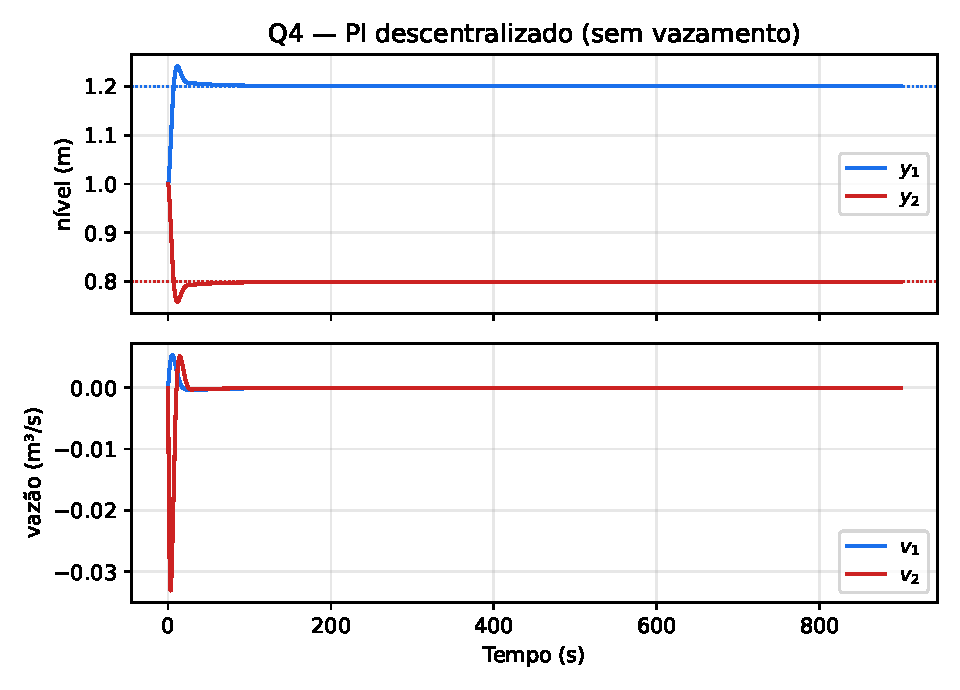
\includegraphics[width=.72\linewidth]{figs/q4_sim.pdf}
\caption{Malha fechada PI descentralizada, refer\^encias compat\'iveis.}
\label{fig:q4sim}
\end{figure}

\subsection*{(f) Modelos com vazamento no tanque 2}

Com vaz\~ao de fuga desconhecida $d\ge0$ no tanque~2, o balan\c{c}o vira
\[
\dot y_1=v_1-v_2,
\qquad
\dot y_2=v_2-v_1-d .
\]
\textbf{Entrada--sa\'ida:}
\[
Y_1(s)=\frac{G_v U_1-G_b U_2}{s},
\qquad
Y_2(s)=\frac{G_b U_2-G_v U_1}{s}\;-\;\frac{D(s)}{s},
\]
i.e.\ o vazamento entra como perturba\c{c}\~ao integrada na sa\'ida 2.
\textbf{Espa\c{c}o de estados:} mesmas matrizes $(A,B,C)$ do item (c) mais a
entrada de perturba\c{c}\~ao
\[
\dot x=Ax+Bu+E\,d,
\qquad
E=\begin{bmatrix}0&0&0&-1\end{bmatrix}^{\!\top}.
\]
A lei de conserva\c{c}\~ao passa a ser $\dot y_1+\dot y_2=-d$: \emph{o volume total
drena \`a taxa $d$, independentemente do controle}.

\subsection*{(g) Capacidade de rejei\c{c}\~ao do vazamento --- an\'alise de sensibilidade}

\textbf{An\'alise malha-a-malha (enganosa).} Cada malha isolada, com PI, tem
fun\c{c}\~ao de sensibilidade $S_i=1/(1+C_ig_{ii})$ com $S_i(0)=0$: a teoria SISO
sugeriria rejei\c{c}\~ao perfeita de perturba\c{c}\~oes constantes.

\textbf{An\'alise estrutural (correta).} A rela\c{c}\~ao
$\dot y_1+\dot y_2=-d$ vale \emph{para qualquer} $u_1,u_2$: a soma dos n\'iveis
\'e n\~ao control\'avel e drena em rampa, $y_1(t)+y_2(t)=w_0-d\,t$. Portanto:
\begin{itemize}[itemsep=1pt]
\item \'E imposs\'ivel (para \emph{qualquer} controlador, descentralizado ou
MIMO) manter os dois n\'iveis simultaneamente: manter $y_1$ exige $v_1=v_2$ e ent\~ao
$\dot y_2=-d$; manter $y_2$ exige $v_2-v_1=d$ e ent\~ao $\dot y_1=-d$. Pode-se
sustentar \emph{um} n\'ivel \`a custa do outro.
\item Com os \emph{dois} PIs ativos, os integradores entram em conflito: cada um
tenta zerar o seu erro, o que \'e incompat\'ivel; as vaz\~oes crescem
(\emph{windup}, at\'e satura\c{c}\~ao dos atuadores) e os dois n\'iveis se afastam
das refer\^encias enquanto $y_1+y_2$ cai em rampa. A simula\c{c}\~ao da
Fig.~\ref{fig:q4leak} (vazamento $d=0{,}005~\mathrm{m^3/s}$ a partir de $t=300$~s)
mostra exatamente isso.
\item Em termos de sensibilidade: a matriz de transfer\^encia de $d$ para
$(y_1,y_2)$ em malha fechada mant\'em um polo em $s=0$ na dire\c{c}\~ao
$[1\;\;1]^{\!\top}$ (modo n\~ao control\'avel), logo o ganho DC de rejei\c{c}\~ao
nessa dire\c{c}\~ao \'e \emph{infinito} (n\~ao rejeita); na dire\c{c}\~ao
$[1\;-1]^{\!\top}$ os PIs rejeitam perfeitamente ($S(0)=0$).
\end{itemize}
\textbf{Conclus\~ao e recomenda\c{c}\~oes:} os controladores propostos rejeitam o
efeito \emph{diferencial} do vazamento, mas nenhum controlador rejeita seu efeito
sobre o volume total --- \'e uma limita\c{c}\~ao da \emph{planta}
(falta um grau de liberdade de reposi\c{c}\~ao de volume), n\~ao da sintonia.
Mitiga\c{c}\~oes: (i)~controlar apenas $y_1$ (ou a combina\c{c}\~ao $y_1-y_2$) e
monitorar $y_2$ com alarme; (ii)~estimar $d$ (observador de perturba\c{c}\~ao,
detec\c{c}\~ao de vazamento pela rampa de $y_1+y_2$); (iii)~mudar a estrutura do
processo, desacoplando a vaz\~ao de sa\'ida do tanque~2 de $v_1$ ou acrescentando
vaz\~ao de reposi\c{c}\~ao --- a\'i sim $G(s)$ ganha posto~2 e o problema se torna
completamente control\'avel.

\begin{figure}[htb]
\centering
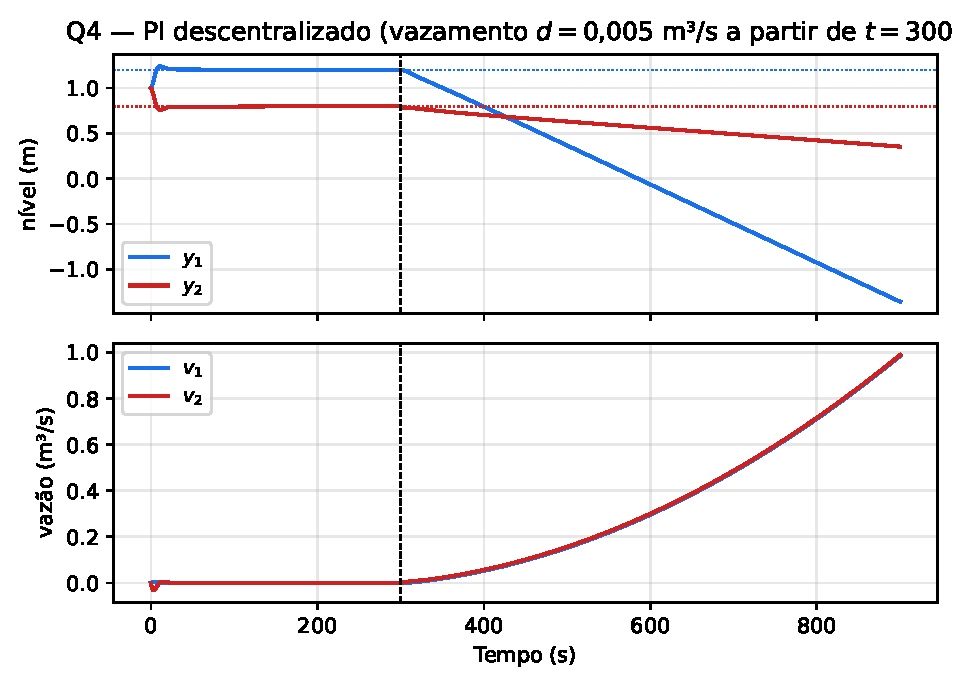
\includegraphics[width=.72\linewidth]{figs/q4_sim_leak.pdf}
\caption{Efeito do vazamento: os integradores conflitam, as vaz\~oes crescem e os
n\'iveis divergem das refer\^encias ($y_1+y_2$ cai em rampa $-d\,t$).}
\label{fig:q4leak}
\end{figure}

\end{document}
